\documentclass{article}
\usepackage{amsmath}
\usepackage[utf8]{inputenc}
\usepackage{float}
\usepackage{epsfig,graphicx}
\usepackage{xcolor,import}
\usepackage[german]{babel}
\usepackage{textcomp}
\usepackage{mathtools}

\begin{document}
\thispagestyle{empty}
			\begin{center}
			\Large{Fakultät für Physik}\\
			\end{center}
\begin{verbatim}


\end{verbatim}
							%Eintrag des Wintersemesters
			\begin{center}
			\textbf{\LARGE WINTERSEMESTER 2014/15}
			\end{center}
\begin{verbatim}


\end{verbatim}
			\begin{center}
			\textbf{\LARGE{Physikalisches Praktikum 1}}
			\end{center}
\begin{verbatim}




\end{verbatim}

			\begin{center}
			\textbf{\LARGE{PROTOKOLL}}
			\end{center}
			
\begin{verbatim}





\end{verbatim}

			\begin{flushleft}
			\textbf{\Large{Experiment Nr.9:} Gleichstrom}\\
							%Experiment Nr. und Titel statt den Punkten eintragen
			\LARGE{}	
			\end{flushleft}

\begin{verbatim}

\end{verbatim}	
							%Eintragen des Abgabedatums, oder des Erstelldatums des Protokolls
			\begin{flushleft}
			\textbf{\Large{Datum:}} \Large{12.12.2014}
			\end{flushleft}
			
\begin{verbatim}
\end{verbatim}
							%Namen der Protokollschreiber
		\begin{flushleft}
			\textbf{\Large{Namen:}} \Large{Veronika Bachleitner, Erik Grafendorfer}
			\end{flushleft}

\begin{verbatim}


\end{verbatim}
							%Kurstag und Gruppennummer, zb. Fr/5
			\begin{flushleft}
			\textbf{\Large{Kurstag/Gruppe:}} \Large{Fr/1}
			\end{flushleft}

\begin{verbatim}






\end{verbatim}
							%Name des Betreuers, das Praktikum betreute.
			\begin{flushleft}
			\LARGE{\textbf{Betreuer:}}	\Large{KLEPP}	
			\end{flushleft}
\newpage	

\section{Photovoltaische Solarzellen als Gleichstromquelle}

\subsection{Aufgabenstellung}
Verschiedene Kenndaten einer Solarzelle werden durch Spannungsmessungen an verschiedenen Stellen in einem Stromkreis ermittelt: Der Kurzschlussstrom $I_{KS}$, die Leerlaufspannung $U_{LL}$, der Kurvenfüllfaktor $CFF$ sowie der optimale Verbraucherwiderstand $R_L$.
\subsection{Grundlagen}
Eine Solarzelle liefert Gleichstrom, was bedeutet das bei wachsendem Verbraucherwiderstand $R_L$ die Spannung ebenfalls wächst - was bei $R_L \rightarrow \infty$ problematisch wird. Die Spannung wächst dann gleichermaßen. Um das zu verhindern werden in Solarzellen intern Dioden eingebaut, die ab einer gewissen Leerlaufspannung $U_{LL}$ beginnen, den Kurzschlussstrom $I_{KS}$ intern abfließen zu lassen. Durch die Konstruktion fließt ständig Strom ab. Man will diesen Verluststrom natürlich gering halten. Dazu wird versucht, den Kurzschlussstrom erst sprungartig ab der Leerlaufspannung abfließen zu lassen. Der Faktor, mit dem dieser Sprung gelingt, wird Kurvenfüllfaktor $CFF$ genannt. Er beschreibt das Verhältnis aus maximal mit der Zelle erreichbaren Leistung und der Leistung zum Kurzzschluss.\\
\begin{equation}
\label{Kurvenfaktor}
CFF=\frac{P_{max}}{I_{KS}\cdot U_{LL}}
\end{equation}
Die Leistung ergibt sich nach dem Ohmschen Gesetz. 
\subsection{Versuchsaufbau und Methoden}
An eine künstlich beleuchtete Solarzelle werden ein Potentiometer und ein Messwiderstand in Serie geschlossen. Zwei Spannungsmessgeräte messen die Gesamtspannung sowie die Spannung am Messwiderstand, um den fließenden Strom zu ermitteln. Diese Methode wird verwendet um uns nicht um den interessanten Fall des Kurzschlusses bei 0 $\Omega$ durch den Innenwiderstand eines Strommessgerätes zu betrügen. Dann wird der Widerstand am Potentiometer in Schritten verändert, bei denen ähnlich große Spannungsänderungen beobachtet werden. Schließlich werden nahe der Leerlaufspannung starke Stromänderungen beobachtet, und nahe des Kurzschlussstroms starke Gesamtspannungsänderungen.\\
Aus dem Plot der Strom-Spannungs-Kennlinie können wir durch Extrapolation den Kurzschlussstrom wenn der Spannung 0 und die Leerlaufspannung wenn der Strom 0 wird ermitteln.\\
Ermitteln wir aus dem Strom und der Spannung die Leistung und plotten diese, finden wir die maximale Leistung und den dazugehörigen Lastwiderstand - durch Vergleich dieser maximalen Leistung mit der Leistung aus dem Produkt des Kurzschlussstroms und der Leerlaufspannung bekommen wir schließlich den Kurvenfüllfaktor CFF.
\subsection{Durchführung}
Wir verwenden zwei Fluke 183 Messgeräte die im Bereich von 5V Gleichspannung mit 5000 Zählimpulsen zu 1 mV auf $\pm (0.07\%$ +1 Zählimpuls) genau messen.
\subsection{Ergebnisse}
Distanz der Solarzelle von der Lichtquelle: 21.5 cm\\
Maximalwiderstand des Potentiometers $R_L$: 1k$\Omega$ \\
Verwendeter Messwiderstand: $R_1$ = 0.517$\Omega$\\
Durch Extrapolation mit SciDaVis, einem qtiplot-fork, konnten wir den Kurzschlussstrom und die Leerlaufspannung ermitteln. \\
In der folgenden Tabelle sind der Kurzschlussstrom $I_{KS}$, die Leerlaufspannung $U_{LL}$, der Kurvenhüllfaktor CFF, der optimale Lastwiderstand $R_L$, sowie die maximale Leistung $P_{max}$ der Solarzelle angegeben.\\
\begin{center}
\begin{tabular}{|c|c|c|c|c|}
\hline 
$I_{KS}$ & $U_{LL}$ & CFF & $R_L$ & $P_{max}$ \\
\hline \hline
(0.049$\pm $0.001)A & (0.93 $\pm$ 0.02)V & (0.661 $\pm$ 0.008) & (17.9 $\pm $0.6) $\Omega$ &(0.030 $\pm$ 0.001) W \\
\hline
\end{tabular}\\
\end{center}
\begin{center}
\begin{figure}
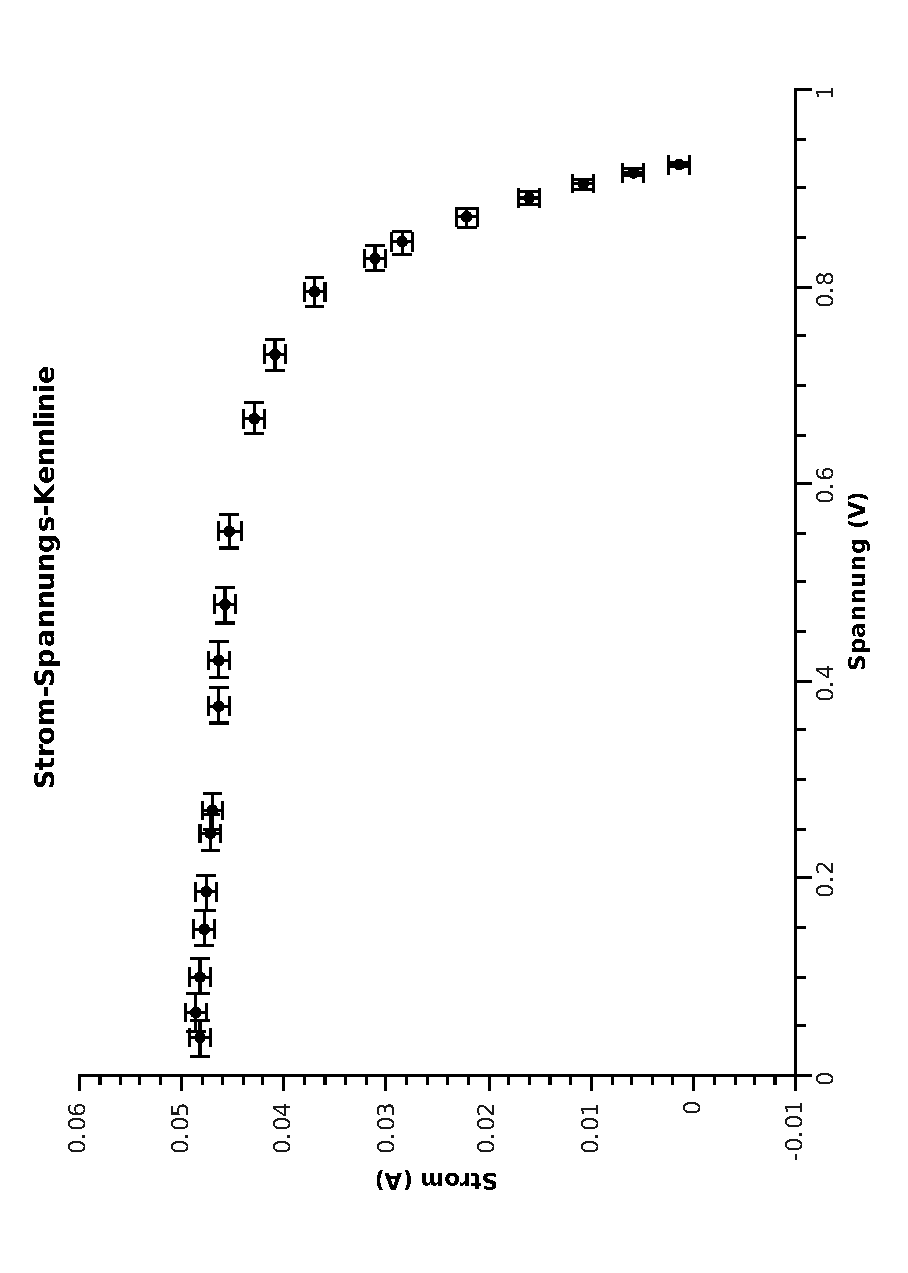
\includegraphics[scale=0.7,angle=-90]{stromspannungsolar.eps}
\end{figure}
\end{center}
\begin{center}
\begin{figure}
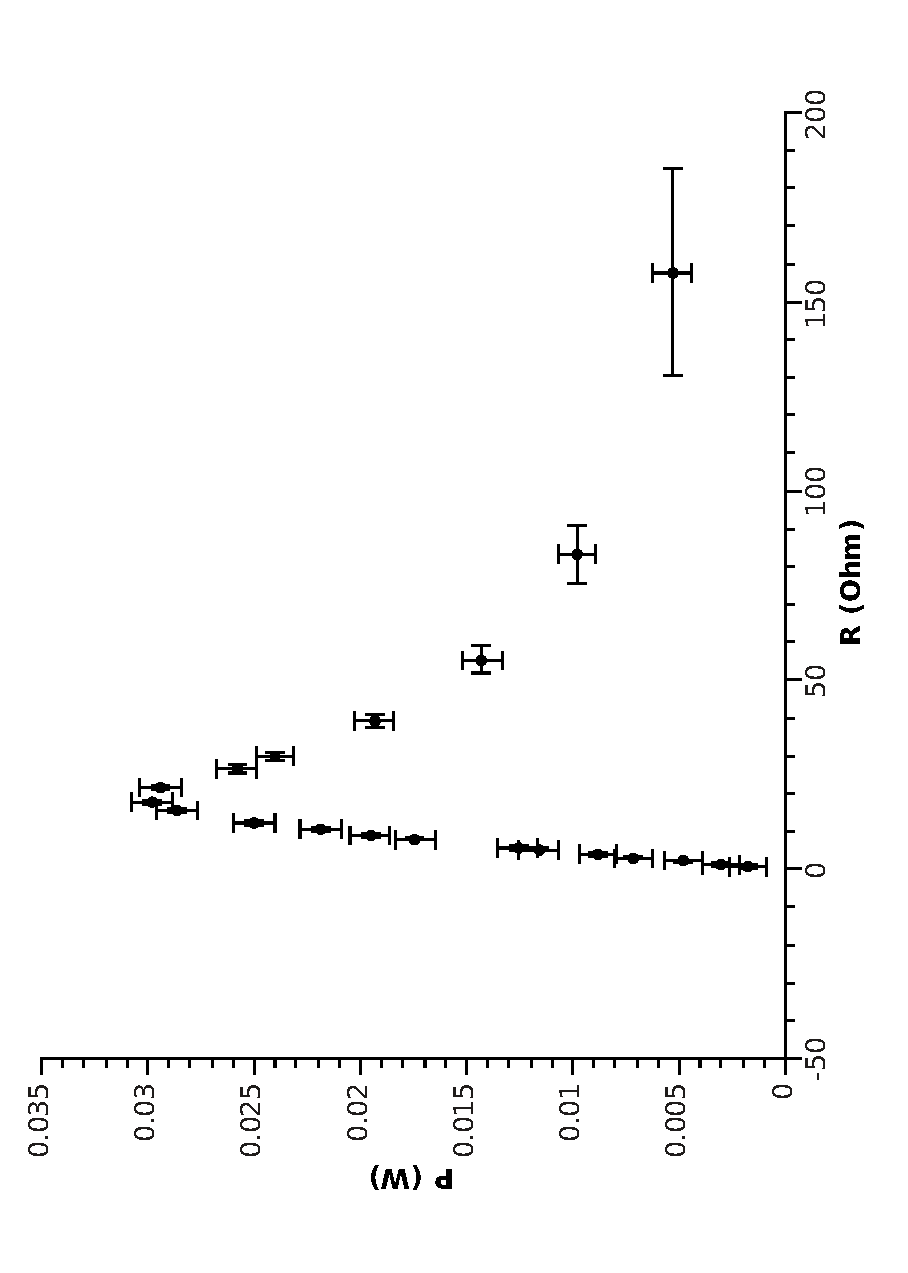
\includegraphics[scale=0.7,angle=-90]{leistung.eps}
\end{figure}
\end{center}
\subsection{Diskussion}
Dadurch, dass bei der Berechnung von CFF die Ausdrücke in Zähler und Nenner mit dem selben Messgerät bestimmt wurden sind ihre Unsicherheiten korreliert und ihre relativen Unsicherheiten konnten subtrahiert werden. Dadurch haben wir ein schön genaues Ergebnis erhalten.


\newpage



\section{Widerstandsbestimmung mittels Wheatstone Brücke}

\subsection{Aufgabenstellung}
Wir messen drei unbekannte Widerstände mit Hilfe einer Brückenschaltung.
Außerdem messen wir den Gesamtwiderstand zweier Widerstände einmal in einer Reihenschaltung und einmal in einer Parallelschaltung und vergleichen unsere Messungen mit berechneten Ergebnissen.
\subsection{Grundlagen}
Eine Wheatstone Brücke ist eine Messungsmethode zur Bestimmung von Widerständen. Sie besteht aus vier Widerständen, die zueinander parallel geschalten werden. 
Von den Widerständen ist einer bereits bekannt ($R_0$), einer wird gesucht ($R_x$) und von den restlichen zweien wird nur das Verhältnis benötigt ($R_a$, $R_b$).\\
Ist dieses Verhältnis genau so groß wie das Verhältnis des unbekannten zum bekannten Widerstand, gibt es keinen Potentialunterschied zwischen den beiden Zweigen. Also ist dort die Spannung gleich null.\\
Mathematisch bedeutet das: $I_1 R_a = I_2 R_x$ und $I_1 R_b = I_2 R_0$. Daraus erhält man: \\
$$R_X=R_0 \frac{R_a}{R_b}$$
und hat so also den gesuchten Widerstand gefunden. 
 
\subsection{Versuchsaufbau und Methoden}
In unserem Experiment handelt es sich bei $R_a$ und $_b$ um einen Schleifdrahtwiderstand. Das Verhältnis der Widerstände $R_a : R_b$ kann man nun auch schreiben als das Verhältnis der Längen $a : b$, da der Draht über die gesamte Länge konstanten Querschnitt und konstanten spezifischen Widerstand hat.\\
\\
Außerdem benötigen wir ein Gleichspannungsnetzgerät (2.3V), ein Ampèremeter, eine Widerstandsdekade (stellt unseren $R_0$ dar) und einen unbekannten Widerstand. 

\subsection{Durchführung}
\subsection{Ergebnisse}
In der Brücke:
RM: 494mm, 7060 Ohm
RF: 475mm, 360 Ohm
RG: 463mm, 1360 Ohm

Testwiderstand R0: 1kOhm
in der Reihenschaltung für die Widerstände G und M: 8.10 k$\Omega$
in der Parallelschaltung für G und M: 1.026 k$\Omega$
\subsection{Diskussion}
\textbf{Zu Fehlerrechnung / Genauigkeit:}
Das Ergebnis wird deswegen genauer, wenn sich der Schieberegler in der Mitter der Widerstandsleiste befindet, weil die Unsicherheit auf der Längenskala eine fixe Größe hat. Prozentuell wird die relative Unsicherheit dann aber umso größer, je kleiner die gemessene Länge ist. 



\newpage



\section{Reale Spannungsquelle}

\subsection{Aufgabenstellung}
Wir nehmen die Strom-Spannungskennlinie einer Batterie auf und bestimmen daraus den Innenwiderstand der Batterie und die Quellenspannung.


\subsection{Grundlagen}
Eine reale Spannungsquelle hat einen endlichen Innenwiderstand. Um das Verhalten der Quelle in einem Stromkreis trotzdem beschreiben zu können, müssen wir iein Ersatzschaltbild machen: Mit einer idealen Quelle, die also keinen Innenwiderstand besitzt, und einen dazu in Serie geschaltenen Widerstand $R_i$.\\
Die Quellenspannung ist die Spannung der idealen Batterie.\\
Der Strom $I=U_0/(R_i+R_L)$ bewirkt einen Spannungsabfall am Innenwiderstand, daher bezeichnen wir die Spannung der realen Batterie (Klemmenspannung): $U_{KL}=U_0-IR_i$.


\subsection{Versuchsaufbau und Methoden}
Aus den Grundlagen finden wir eine Methode, den gesuchten Innenwiderstand der Batterie zu bestimmen:\\
Wir messen die Klemmenspannung als Funktion des Stromes: $U_{KL}=U_{KL}(I)$. Die Steigung der resultierenden Gerade ist gleich $R_i$.\\
Weiters kann die Quellenspannung $U_0$ durch Extrapolation bestimmt werden.\\
\\
Wir verwenden eine Batterie, ein Volt- und ein Ampèremeter (beides Fluke 183), eine Widerstandsdekade als Lastwiderstand und einen Taster zum Öffnen/Schließen des Stromkreises.\\
\\
\textbf{Unsicherheiten der Messgeräte:} \\
Ampèremeter - Fluke 183:\\
Auflösung: $100\mu A$\\
Genauigkeit: $\pm$ (0,2\% + 4 Zählimpulse)\\
\\
Voltmeter - Fluke 183:\\
Auflösung: $1mV$\\
Genauigkeit: $\pm$ (0.07\% + 1 Zählimpuls)


\subsection{Durchführung}
Wir messen die Leerlaufspannung mit offenem Taster. Sie verändert sich während unserer Messung vernachlässigbar; um 0.001V.\\ 
Anschließend messen wir $U_{KL}$ und $I$ mit variablen Widerständen. Wir gehen dabei in Schritten von $20\Omega$ von 200$\Omega$ bis $20\Omega$.\\
Die Daten werten wir mit QTI-Plot aus.

\newpage
\subsection{Ergebnisse}
Leerlaufspannung: 1.505V\\
\\


\begin{tabular}{|r|l|l|}
\hline
$R_L$ $[\Omega]$ & Spannung U [V] & Strom I [mA]\\
\hline
200 & 1.494 $\pm$ 0.002 & 7.43 $\pm$ 0.055\\
180 & 1.494 $\pm$ 0.002 & 8.26 $\pm$ 0.057\\
160 & 1.492 $\pm$ 0.002 & 9.27 $\pm$ 0.059\\
140 & 1.491 $\pm$ 0.002 & 10.59 $\pm$ 0.062\\
120 & 1.489 $\pm$ 0.002 & 12.32 $\pm$ 0.065\\
100 & 1.487 $\pm$ 0.002 & 14.73 $\pm$ 0.070\\
80 & 1.483 $\pm$ 0.002 & 18.33 $\pm$ 0.077\\
60 & 1.477 $\pm$ 0.002 & 24.27 $\pm$ 0.089\\
40 & 1.466 $\pm$ 0.002 & 35.94 $\pm$ 0.12\\
20 & 1.445 $\pm$ 0.002 & 69.20 $\pm$ 0.18\\
\hline
\end{tabular}


\begin{center}
\begin{figure}[H]
\includegraphics[scale=0.5]{batterie_kennlinie.eps} 
\end{figure}
\end{center}

QTI-Plot gibt uns für den Fit mittels $y=Ax+B$ (wobei y: Spannung U, x: Strom I) die folgenden Werte: 
\begin{quote}
From $x = 7.43$ to $x = 35.94$\\
$a  = -0.000995923244694066 \pm 1.39673189659993e-05$\\
$b  = 1.50150717852846 \pm 0.000251022348126121$\\
-------------------------------------\\
$R^2 = 0.998625088078122$\\
\end{quote}


\newpage
Unser Ergebnis für den Innenwiderstand der Batterie ist der Wert der Variable a mal 1000. (Da wir für den Strom mA verwendet haben.)\\
$$\boxed{R_i=(0.996 \pm 0.014)\Omega}$$\\
\\
Unser Ergebnis für die Quellenspannung ist der Wert der Variable b. \\
$$\boxed{U_0=1.50151 \pm 0.00026}$$


\subsection{Diskussion}
\textbf{Eine Anmerkung zu unseren Unsicherheiten:}\\
Bei der Strommessung ist uns aufgefallen, dass bei einigen Werten die Unsicherheit mit der Rundung auf 2 relevante Stellen eine Nachkommastelle mehr besitzt als unser eigentlicher Wert.\\
Wir überprüfen also, ob eine Rundung auf eine Stelle weniger sinnvoll ist. Dies taten wir nach Anleitung aus der Vorlesung "Auswertung und Dokumentation experimenteller Daten" und sehen daraus, dass wir eine zusätzliche Rundungssicherheit von 11\% im Maximum erhalten würden. Daher belassen wir die Unsicherheiten wie sie sind.\\
\\
\textbf{Zu den Ergebnissen:}\\
Wir ignorieren den Wert $I=69.20$ bei der Erstellung der Stroms-Spannungs-Kennlinie, da dieser den linearen Fit hebelt. Der Wert ist beinahe doppelt so groß wie der vorhergehende. Wir erklären uns dies dadurch, dass der Widerstand hier schon sehr klein ist und wir uns bei den $20\Omega$ schon nahe am Kurzschluss befanden.
\\
Das Ergebnis für den Innenwiderstand $R_i\approx 1\Omega$ ist laut unserem Betreuer passend.\\
Die Quellenspannung entspricht wie erwartet etwa der gemessenen Leerlaufspannung.

\newpage

\section{Belasteter Spannungsteiler}

\subsection{Aufgabenstellung}
Wir bestimmen aus einer einfachen Schaltung, dem Spannungsteiler, die elektrischen Widerstände von drei Lastwiderständen mit zwei Spannungsmessgeräten.
\subsection{Grundlagen}
Wenn ein Potentiometer seinen Gesamtwiderstand R aufteilt in $R_1$ und (R-$R_1$), erhält man mittels der Kirchhoffschen Regeln für einen Lastwiderstand $R_L$ der zu $R_1$ parallel geschalten ist folgende Beziehung: 
\begin{equation}
\label{spannungsteiler}
\frac{U_L}{U}=\frac{R_1R_L}{R_LR+R_1(R-R_1)}
\end{equation}
$U_L$ bezeichnet die Klemmenspannung am Lastwiderstand $R_L$, U die Gesamtspannung. Wir führen weitere Bezeichnungen ein:
\begin{align*}
r_L=\frac{R_L}{R} \\
r_1=\frac{R_1}{R} \\
u = \frac{U_L}{U}
\end{align*}
Mit diesen erhalten wir schließlich für den Lastwiderstand $R_L$:
\begin{equation*}
r_L=-\frac{u\cdot r_1(1-r_1)}{u-r_1}
\end{equation*}
\begin{equation}
\label{spannungsteiler_umgeformt}
R_L=-R\cdot \frac{u\cdot r_1(1-r_1)}{u-r_1}
\end{equation}

\subsection{Versuchsaufbau und Methoden}
Wir schalten einen Lastwiderstand parallel zu einem Teilwiderstand eines Potentiometer und in Serie zu seinem anderen Teilwiderstand und messen mit zwei gleichen Spannungsmessgeräten die Spannungen am Teilwiderstand und an allen Widerständen. Mit (\ref{spannungsteiler}) und dem Verhältnis der Teilwiderstände am Potentiometer ermitteln wir dann den Lastwiderstand. 
\subsection{Durchführung}
Wir verwenden zwei Fluke 183 Multimeter, die im Bereich von 5V Gleichspannung mit 5000 Zählimpulsen zu 1 mV auf $\pm (0.07\%$ +1 Zählimpuls) genau messen.
\subsection{Ergebnisse}
Wir präsentieren unsere Messergebnisse in der Grafik mit Fehlerbalken:
\begin{center}
\begin{figure} [H]
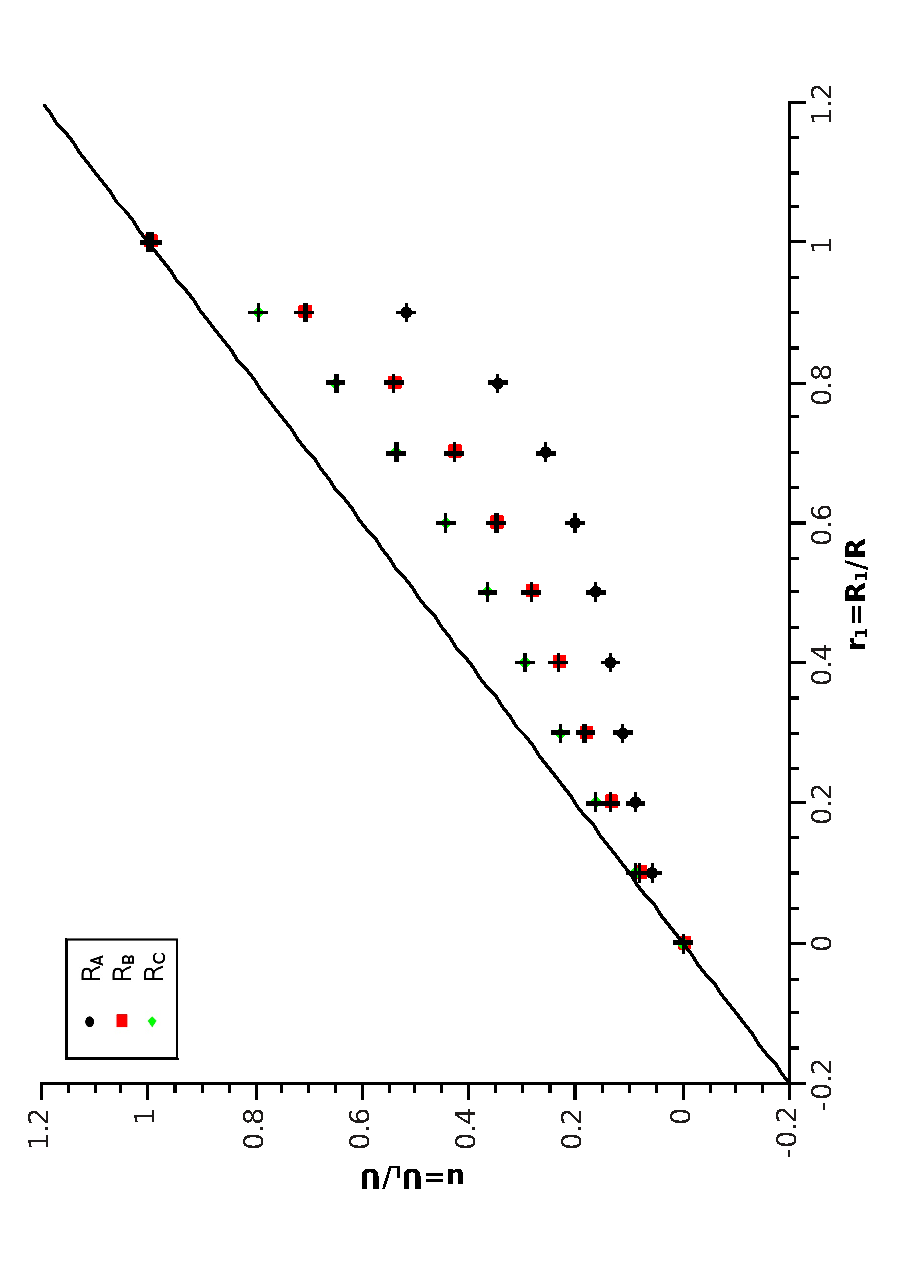
\includegraphics[scale=0.5,angle=-90]{spannungsteiler.eps}
\end{figure}
\end{center}
Daraus erhalten wir mit der Formel (\ref{spannungsteiler_umgeformt}) und Größtfehlerabschätzung für die getesteten Widerstände, wobei wir annehmen dass $\Delta r_1$=0.001 ist:

$$R_A=(1221\pm6) \Omega$$
$$R_B=(3321 \pm 11) \Omega $$
$$R_C=(6831 \pm 31) \Omega $$

Die relative Unsicherheit aller Messwerte beträgt $\approx$ 0.5 \%.
\subsection{Diskussion}
Wenn wir eine Unsicherheit für $\Delta r_1$ von 0.01 annehmen, was wegen dem Bestimmen des von der Mediane fernsten Punkts durch Augenmaß möglicherweise sinnvoll ist, wird die relative Unsicherheit der getesteten Lastwiderstände 8\% groß, im Vergleich zu  0.5 \%. \\
\end{document}
